\section{Model robustness and drift detection}
    In this chapter the stability and robustness of the trained models are presented. First subsection shows models' performance on the corrupted DIC input data with two sources of corrupted signal: artificial pseudocorruptions and real corruptions from the microscope settings. It presents the influence of augmentations on the robusteness, studies the influence of corruptions on practical biological metrics and shows how generalizable the models are across phenotypes. Second subsection presents a study of the image representations in the UNet embeddings including their possible clustering in the lower dimensional space based on several possible clustering hypotheses. And finally the last subsection covers the results of the drift detection algorithm built to alert end users when models predictions become unreliable. Which happens when there is a difference between the data used for training and the data used during inference. 
    
\subsection{Corruptions}  
    For practical reasons it is important to not only evaluate the models on high-quality data exclusively, but also to know how the predictions will degrade when the input's data quality decreases. Having a model for fluorescence \textit{in silico} labeling that can additionally alarm end users when the predictions should not be relied upon is very useful in practice. Although the DIC microscopy is a relatively easy technique, there are still setting up procedures taking place that can be prone to errors. Additionally, as the models are not easily generalizable across phenotypes as well as between fixed and not fixed cells, an alarming system that is able to catch these situations would be useful to save time and cost of lab work. In order to measure the stability or robustness of the models towards data degeneration they were evaluated on the corrupted or "bad" input DIC images. There are two sources of "bad" images that can be used for such estimations. The first are actually corrupted images made in the laboratory. Such corruptions may come from different sources: for example, an oil bubble landed on the microscope lenses, low density of the cell on the image, over- or underexposure during image acquisition. Another source of image corruption would be images with artificial or pseudocorruptions created manually via image processing. They allow more systematic investigation of the impact of a corruption effect. Artificial corruptions allow to vary the severity of the corruption keeping the original fluorescence data intact.
    
    %This chapter first provides a description of artificial corruptions used to evaluate previously trained models on. Afterwards the real examples of corruptions acquired from the lab are 
    \subsubsection{Artificial corruptions}
        
In this subsection results from evaluating models on 3 types of artificial image corruption are presented, namely: defocus blur imitating the defocus of the microscope lenses, changes in brightness and changes in contrast. Every corruption  has different effects on the prediction of the model based on its severity level. Therefore it is important to evaluate the error-rate (in this case a loss function) for the predictions for different severity levels of each of corruption types presented. It is also important to perform a visual evaluation of model's predictions on corrupted data. Each corruption $c$ will have different severity levels $s$, $-5 \leq s \leq 5$ ($0 \leq s \leq 5$ for defocus blur corruption), where $0$ corresponds to original image without corruption. It is important to keep in mind that although severity levels were chosen to be as much comparable between each other as possible, they still might have differences in their strength. For example, contrast has much stronger effect on predictions than brightness changes. Three types of artificial image corruption are presented below.

\subsubsection{Defocus Blur}
Defocus blur corruption imitates the effect of defocus on the microscope. The blur is applied to the image by convolving it with a special defocus kernel. There are two tunable parameters for this corruption type: first one is the readius of the circle in the kernel $r$, and the second one is the blur strength parameter $s$. Examples of the kernel with radius $r$ is shown in the Figure \ref{fig:defocus-blur-kernel}. Such kernel is then simply applied to an image via $cv2.filter2D$ function.

\begin{figure}[htb]
	\begin{center}
		\includegraphics[width=0.2\linewidth]{bilder/stability/defocus-blur-kernel.png}
		\caption{Defocus blur kernel}\label{fig:defocus-blur-kernel}
	\end{center}
\end{figure}

\subsubsection{Brightness}
Different brightness levels are also an important image corruption to test on. Different brightness levels appear often in the dataset during image accquisition. In oder to change the brightness, an image from the RGB format was translated into HSV format, which stands for hue, saturation and value. This is also one of popular formats to represent an image. To make an image brighter or darker, one can simply add or subtract a parameter $s$ in a value channel for each of the pixels correspondingly. This parameter is often called bias. The bigger absolute value of this change the stronger a corruption will be.

\begin{equation}
    \hat{x}_{i, j} = x_{i, j} + s
\end{equation}

\subsubsection{Contrast}
In contrast to adding a constant value pixelwise to an image in order to change a contrast level one can perform a multiplication of an image with another constant $s$. This parameter is often called gain.

\begin{equation}
    \hat{x}_{i, j} = s * x_{i, j}
\end{equation}

For both contrast and brightness changes one can use $cv2.convertScaleAbs()$ from OpenCV library. This method directly accepts gain and bias parameters and clips the image to stay within the allowed values range.

The values of hyperparameters use in corruptions (kernel radius, gain and bias) are streched across the range of severity levels and presented in Table \ref{table:corruption-hyperparameters}.
\begin{table}[H]
    \centering
    \caption{Hyperparameterization for different artificial corruption severities}
        \begin{adjustbox}{width=1\textwidth}
            \begin{tabular}{|l||*{11}{c|}}\hline
                \backslashbox{Corruption}{Severity}
                &\makebox[3em]{-5}
                &\makebox[3em]{-4}
                &\makebox[3em]{-3}
                &\makebox[3em]{-2}
                &\makebox[3em]{-1}
                &\makebox[3em]{0}
                &\makebox[3em]{1}
                &\makebox[3em]{2}
                &\makebox[3em]{3}
                &\makebox[3em]{4}
                &\makebox[3em]{5}
                \\\hline\hline
                Defocus blur (radius) &-&-&-&-&-&0&0.5&1.0&1.5&2&3\\\hline
                Contrast (gain) &3.5&3.0&2.5&2.0&1.5&1&0.9&0.8&0.7&0.5&0.3\\\hline
                Brightness (bias) &-150&-135&-120&-90&-50&0&50&90&120&135&150\\\hline
            \end{tabular}
        \end{adjustbox}
    \label{table:corruption-hyperparameters}
\end{table}

Severity level of $-5$ for contrast represents an highly contrastive image, while $5$ is a very low contrast image. For brightness corruption levels of $-5$ and $5$ correspond to images with very low and high brightness respectively. And defocus blur corruption has only 5 levels of severity from original image (level $0$) to the image with a stronger blur (level $5$).
\begin{figure}[H]
	\begin{center}
		\includegraphics[width=0.5\linewidth]{bilder/corruptions.png}
		\caption{Influence of artificial corruptions on the predictions}\label{fig:artificial-corruptions}
	\end{center}
\end{figure}

One can observe input image change for each of the corruptions along with the change of prediction of nuclei model on these crops. One can clearly notice that model's predictions are quite stable towards different brightness levels and contrast. However, the predictions on the crops are very sensible towards defocus blur corruption: corruptions of levels $1-4$ are almost indistinctable from the original image, yet the model predictions degrade quite soon. This can be explained by fact that training dataset contains quite diverse data in terms of contrast and brightness levels and, as the result, the model is more stable towards these changes. Using defocus blur as an augmentation will help to solve this problem. This will be described in more detail in Section \ref{section:augments-againts-corruptions}.
\begin{figure}[H]
	\begin{center}
		\includegraphics[width=0.5\linewidth]{bilder/corruptions-loss.png}
		\caption{Change of PCC loss for artificial corruptions}\label{fig:corruptions-loss}
	\end{center}
\end{figure}

Additionally, a change in PCC loss is presented in Figure \ref{fig:corruptions-loss}. This is a plot of PCC loss for different artificial corruptions. The loss is increased for stronger severity levels. We can see that in positive direction with defocus blur corruption the model degerates more quickly and that contrast corruptions change prdictions more sever in the negative one.
    \subsubsection{Real corruptions}
        \label{section:real-corruptions}
        Another interesting set of experiments was conducted on the image data that exhibits real corruptions that can happen in the lab due to the wrong settings of the microscopy image acquisition approach. The following data was considered: 
\begin{figure}[htb]
	\begin{center}
		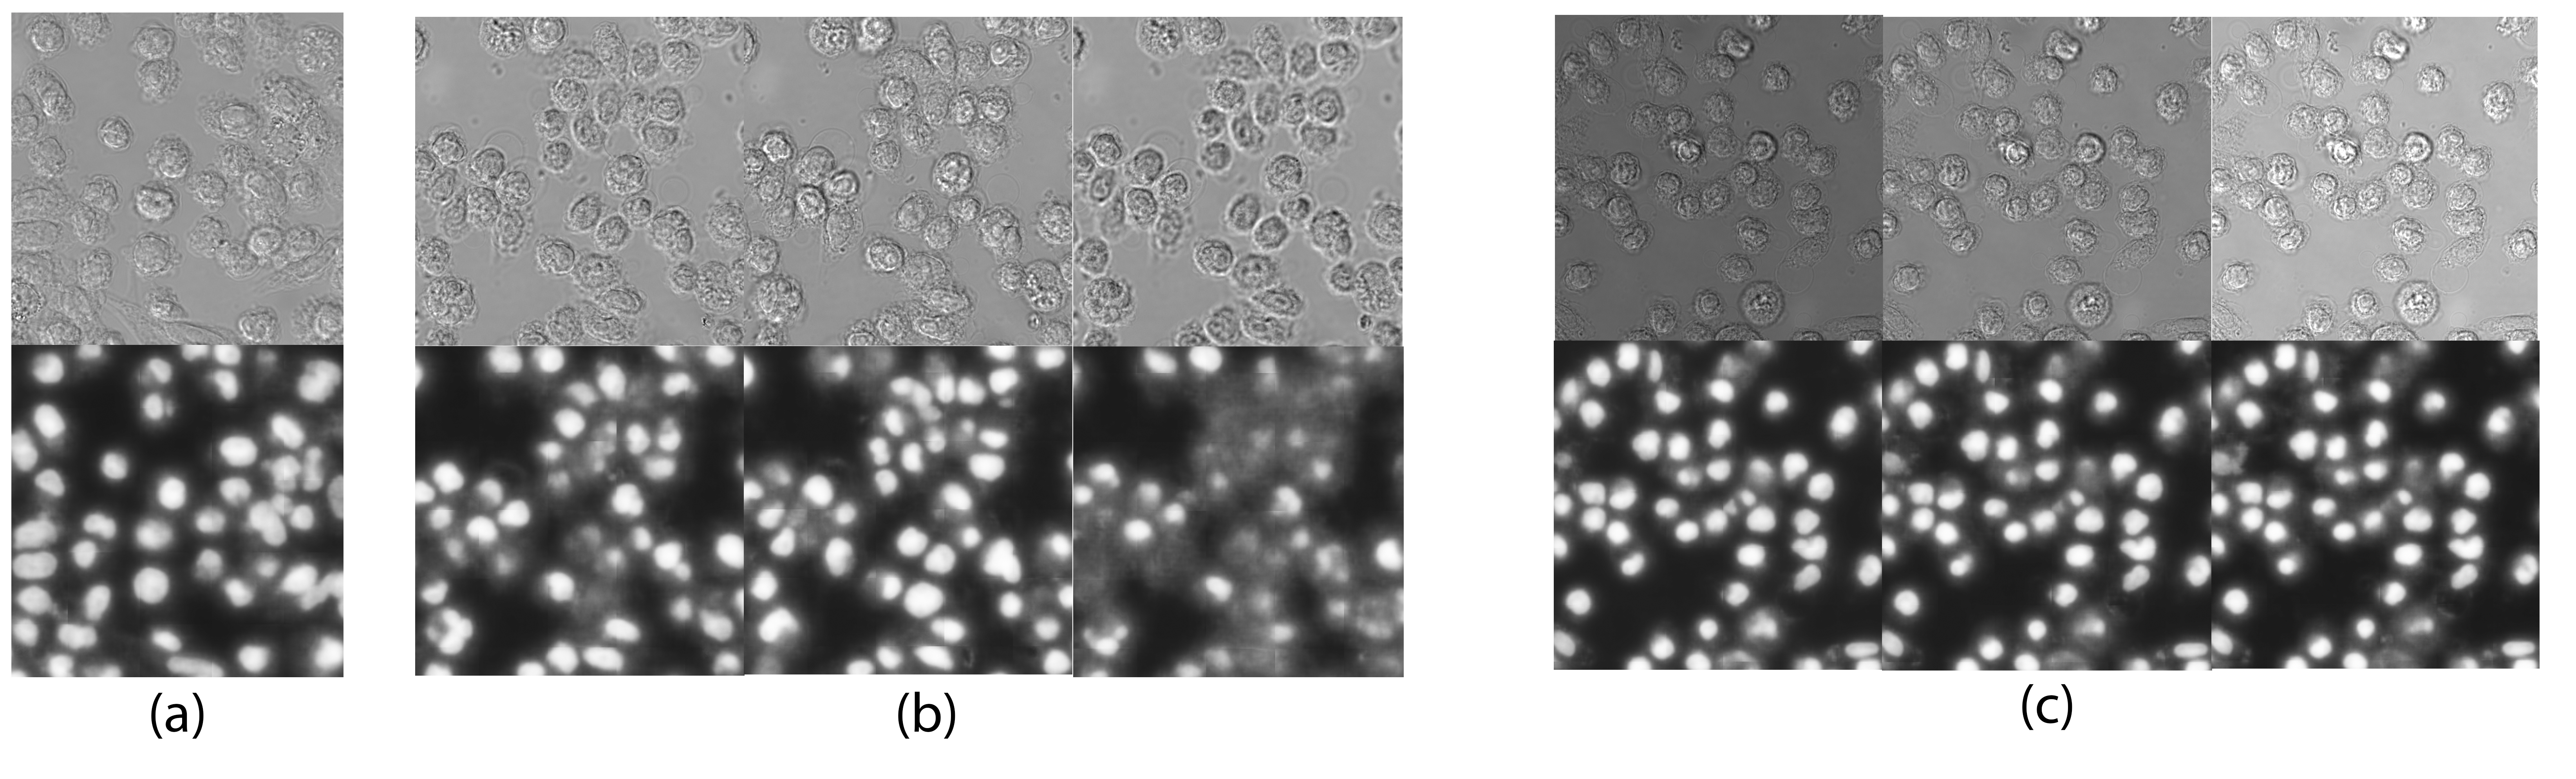
\includegraphics[width=\linewidth]{bilder/drift-detection/real corruptions/predictions.png}
		\caption[]%
		{Real corrupted data from the lab. (a) --- an example of the fixation of the cells in formalin for 15 minutes instead of the usual 10; (b) --- the same image with different microscope focus adjusments. From left to right: microscope stage lowered by 5 microns bringing the subject out of focus, normal height, higher microscope stage by 5 microns bringing the subject out of focus again but in the other direction; (c) --- the same image with different exposure times. From left to right: 20ms --- underexposure, 30ms --- normal setting, 40ms --- overexposure.}\label{fig:real-corruptions-predictions}
	\end{center}
\end{figure}


\begin{itemize}
    \item Figure \ref{fig:real-corruptions-predictions} (a) Wrong fixation time of the cells in formalin. These cells are more turbulent and more strongly clumped together. This is a good example of an image that cannot be simulated artificially with image processing.
    
    \item Figure \ref{fig:real-corruptions-predictions} (b) A real example of a defocus blur from the microscope, when microscope stage was lowered or elevated by 5 microns bringing the subject out of focus.
    
    \item Figure \ref{fig:real-corruptions-predictions} (c) A real example of contrast / brightness differences due to wring exposure times.
\end{itemize}

The model tested here is the model trained on nucleus with simple augmentations (scale, rotation, flips). From Figure \ref{fig:real-corruptions-predictions} it can be concluded that the time of formalin fixing does not really matter for nucleus outline, however the amount of details inside the nuclei seems to be slightly higher than with the usual fixation procedure. Focus of the microscope is clearly very important for good predictions. Although the negative direction of the focus loss seems to have better predictions than the positive one, many of the nuclei are simply gone in the fluorescence image in both cases. Over- and underexposure do not influence the predictions that drastically. Visually different exposure seems to change image brightness and the model is stable towards these changes. Nucleus outline stays mostly the same here as well, but the shining around it is dependent on the exposure times.
    \subsubsection{Improving predictions with additional corruption augmentations}
        \label{section:augments-againts-corruptions}
        \begin{figure}[htb]
	\begin{center}
		\includegraphics[width=0.4\linewidth]{bilder/stability/augments-help.png}
		\caption{Using corruptions as augmentations improves predictions}\label{fig:augments-help}
	\end{center}
\end{figure}

    \subsubsection{Generalizability across phenotypes}
        TODO train the model on one phenotype and predict on the other, compare predictions (visually?)
        postprocessing with metrics then?
    \subsection{UNET embeddings study}
    Similarly to studying autoencoder embeddings that represent a high-dimentional input in lower dimentional space, one can study UNet embeddings. However, it is important to keep in mind that the dimensionality of embeddings in UNet case is not lower than dimensionality of the input and is even often higher (see the UNet architecture in Figure \ref{fig:unet}). The goal of a UNet in contrast to an autoencoder is not to compress the input, but to extract useful features that are helpful for high-resolution segmentation. UNet embeddings do not contain rich image semantics in them as embeddings of an autoencoder do. UNet compresses the spatial dimention of the input, but at the sme time it gradually increases the number of filters that capture of information need for segmentation. As it has been proven in section \ref{section:nuclei-predictions} having more filters only helps to get better predictions, therefore there is no need for a UNet to have low-dimentional embeddings. Nevertheless, it is still interesting to see if the embeddings do contain any information about the input that one could use. There were two hypothesis put in question: the first one is whether embeddings of a trained UNet form any kind of clusters based on cells phenotype. And a second one is whether embeddings of corrupted images can be clustered together further away from not corrupted ones. If the latter hypothesis would hold, one could alarm the end-user about the outliers in the dataset based on their distance from both of the clusters. 
    \subsubsection{Application of various dimentionality reduction methods}
        \label{section:unet-embeddings-dim-reduction}
        It is important that any image is fed into the network crop by crop, meaning that for each crop there is a separate embedding. In this section crops embeddings were not combined in any way together and were analysed separately.

The UNet embedding has a size of $16 \times 16 \times 256$ and can be flattened into a $655536$-dimensional vector. In order to comprehend the embeddings for us as humans, a dimensionality reduction algorithm has to be applied. One option would be to compress a vector to 2D or 3D representation, which is easily comprehendable by humans.
\begin{figure}[htb]
	\includegraphics[width=\linewidth]{bilder/unet-embeddings/umap-pca-embeddings.png}
	\caption[Visualization of UNet embeddings in 2D space]%
	{Visualization of UNet embeddings in 2D space. (a) PCA, (b) UMAP, (c) combination of PCA and UMAP with 10 and (d) 200 components. First row differentiates between two cell phenotypes: CHOZN and PHX, whereas the second row differentiates between uncorrupted crops and crops corrupted using artificial defocus blur of severity level $4$.}\label{fig:umap-pca-embeddings}
\end{figure}

In this case a two-dimensional representation was chosen. With the help of PCA, UMAP and their combination embeddings were projected into a 2D space. In Figure \ref{fig:umap-pca-embeddings} we can see kernel density estimate (KDE) plots, that were created based on scatter plots, where each dot represents a projected UNet embedding of a crop. Both research questions are addressed here: clustering based on phenotypes (CHOZN or PHX) and clustering based on input corruptions (defocus blur of severity level $4$). It is crucial here that corrupted data was not used in training of any of dimensionality reduction method. The goal was to use only the data available in training dataset, find the transformation of high-dimensional data into a lower-dimensional space and apply it to new samples. That is also why methods like t-sne (\cite{t-sne}) cannot be used here, because the transformation that t-sne learns cannot be applied to new samples. 

From Figure \ref{fig:umap-pca-embeddings} it becomes evident that there is no clustering based on the phenotype. On the one hand, this means that it is not possible to detect phenotype based on the UNet embedding. But on the other hand, this also implies that PHX or CHOZN phenotypes do not influence the predictions so much supports previous conclusion from Section \ref{section:generalizability-across-phenotypes} that the model generalises well across them. Regarding the clustering based on the artificial corruption it seems that embeddings of corrupted samples tend to clump more in groups, occupying one specific area of the embeddings space. It is also clear that the combination of UMAP with previously applied PCA works better with the increasing amount of components in PCA: dots in (d) seem to form a better cluster than dots in (c). However, it can still not be taken intuitively from this figure how many non-corrupted dots are hidden behind the cluster of the green dots --- meaning whether non-corrupted crops cluster intersects severely with a corrupted one. In order to visualize this better, one can use a kernel density estimate (KDE) plot presented in Figure \ref{fig:kde}. Additionally, it is clear that pure UMAP is not the best approach for the extreme number of dimensions as with the one in this case.

%\begin{figure}[htb]
%	\begin{center}
%		\includegraphics[width=0.6\linewidth]{bilder/unet-embeddings/kde.png}
%	\caption{KDE plot of UMAP applied after PCA with 200 components}\label{fig:kde}
%	\end{center}
%\end{figure}

A cluster of corrupted images is clearly present here, however it also intersects with many non-corrupted crops. The quantitative evaluation of how this cluster is separable from the rest of the points is provided in section \ref{section:clustering-on-unet-embeddings}. Although one can already state that there is a clear opportunity to differentiate between corrupted and not corrupted images, the accuracy cannot be high due to the clusters being not well separable. For further research it is suggested to additionally check whether clusters form into a high-dimensional space before projecting them into a 2D space. 

\paragraph{Clustering with PaCMAP}
\label{section:clustering-on-unet-embeddings}
\begin{figure}[htb]
	\begin{center}
		\includegraphics[width=\linewidth]{bilder/unet-embeddings/PacMAP.png}
		\caption{Clustering of UNet Embeddings}\label{fig:unet-clustering}
	\end{center}
\end{figure}

\begin{figure}[htb]
	\begin{center}
		\includegraphics[width=0.6\linewidth]{bilder/unet-embeddings/db-levels.png}
		\caption{Clustering for different severities levels}\label{fig:unet-clustering-sev-levels}
	\end{center}
\end{figure}

TABLE with F1-score:
0.76 VS 0.64

    \subsubsection{Autoencoder embeddings as an alternative}
        Since UNet embeddings seem to not exhibit any exceptional results in termns of clustering, it was decided to train a vanilla autoencoder directly on image crops. Since autoencoder's embeddings contain dense semantic information of the input they might provide more insights for clustering hypotheses mentioned before. Figure \ref{fig:ae-training} presents the architecture of two convolutional autoencoders used for these experiments. One compresses $256 \times 256$ input crops into embeddings vector of size $3528$ and another one compresses them into a vector of a smaller size $200$. Both autoencoders were trained using MSE loss. The results of their convergence are presented in Figure \ref{fig:ae-training} on the right.

\begin{figure}[H]
	\begin{center}
		\includegraphics[width=\linewidth]{bilder/ae-embeddings/training-architectures.png}
		\caption{Architectures of two autoencoders and their training convergence}\label{fig:ae-training}
	\end{center}
\end{figure}

An autoencoder with embeddings of bigger size was able to achieve a lower loss as well as samples reconstructed from it were of a better quality (see Figure \ref{fig:ae-samples}). Clearly samples reconstruction will not have a high resolution as there are no skip-connections in this architecture. However, this is also not needed, the main goal here would be to find out whether autoencoder embeddings provide any insights on the data.
\begin{figure}[H]
	\begin{center}
		\includegraphics[width=0.5\linewidth]{bilder/ae-embeddings/ae-samples.png}
		\caption{Samples drawn from trained autoencoders}
		\label{fig:ae-samples}
	\end{center}
\end{figure}

Since an autoencoder with bigger embeddings size seems to be able to reconstruct crops much better we have proceeded with its achtitecture. Embeddings were projected into a 2-dimensional space using first PCA with 10 components and then applying UMAP on PCA's projections. The results of such projection are presented in Figure \ref{fig:ae-pca-umap-clustered}. Two clearly defined clusters appear: left plot presents projections from an earlier epoch, the right one --- from a later one. Embeddings separate gradually into two clusters throughout the training.

\begin{figure}[htb]
	\begin{center}
		\includegraphics[width=0.8\linewidth]{bilder/ae-embeddings/pca-umap-clusters.png}
		\caption{Autoencoder embeddings after applying PCA with 10 components and UMAP afterwards. Earlier epoch VS later epoch.}\label{fig:ae-pca-umap-clustered}
	\end{center}
\end{figure}

However, these two clusters are based neither on cell phenotype nor on input corruption. All points of both phenotype as well as corruptions seem to be equally mixed between two custers. By looking at the images correponding to each of the clusters it soon became clear that the main difference between them is their brightness level. To prove this theory distirbutions of average image intensity of images in both clusters are presented in Figure \ref{fig:ae-brighter-darker}. From violin plots it becomes clear that distribution of the crops on the left has a much lower brightness level than distribution of the crops on the right.
%\begin{figure}[htb]
%	\begin{center}
%		\includegraphics[width=0.5\linewidth]{bilder/ae-embeddings/pacmap.png}
%		\caption{PacMAP does not provide information on the coruption}\label{fig:ae-pacmap}
%	\end{center}
%\end{figure}

\begin{figure}[H]
	\begin{center}
		\includegraphics[width=0.5\linewidth]{bilder/ae-embeddings/brighter-darker.png}
		\caption{What do two UMAP clusters represent}
		\label{fig:ae-brighter-darker}
	\end{center}
\end{figure}

Since an autoencoder picks up on brightness difference within the crops, it is worth trying to normalize crops brightness across all dataset first. Nevertheless, it is not a trivial task as images have different cell density in them. That is why some images that contain primarily background pixel will always be darker than the ones that contain enough of foreground. We suggest to filter the crops based on amount of cells critea (which can be done using GFP model that can detect cells present in DIC) and normalize them afterwards. Retraining autoencoder on new training data might provide more insights when difference in brightness will be gone.

It is also clear why autoencoder embeddings do not provide any clustering for corrupted crops. Corruption severities neither really change the image semantics nor they are significantly different visually (see defocus blur in \ref{fig:artificial-corruptions}). Therefore they do not alter the ability of an autoencoder to restore input correctly. In contrast, UNet's fluorescence predictions do suffer significantly for severy corruption levels, its predictions strongly changes --- outline of the organelle becomes more blurry, additional shine appears in fluprescence prediction. These changes happen not only during the decoding part, but they also might bring unsual values in the embedding representation. Therefore when UNet embeddings have more information on the "trustworthiness" of predictions. That is why when defocus corruptions are used as training augmentations, drift detection for the model trained with these corruptions stops alarming about the drift, although it did for the model, which did not have these augmentations present TODO add reference. This happens simply because models predictions degrade and start looking different, which triggers a "drift alarm", with the imroved predictions, drift alarm would not be triggered even when using the same data.
    \subsubsection{Clustering of PacMAP embeddings}
        \paragraph{Clustering on UNet embeddings}
        \label{section:clustering-on-unet-embeddings}
        \begin{figure}[htb]
	\begin{center}
		\includegraphics[width=\linewidth]{bilder/unet-embeddings/PacMAP.png}
		\caption{Clustering of UNet Embeddings}\label{fig:unet-clustering}
	\end{center}
\end{figure}

\begin{figure}[htb]
	\begin{center}
		\includegraphics[width=0.6\linewidth]{bilder/unet-embeddings/db-levels.png}
		\caption{Clustering for different severities levels}\label{fig:unet-clustering-sev-levels}
	\end{center}
\end{figure}

TABLE with F1-score:
0.76 VS 0.64
    \subsubsection{Embeddings for direct stability prediction}
        The problem of substituting fluorescence labeling with \textit{in silico} prediction solved in thesis is a step towards a general goal of the project within Merck KGaA oriented towards predicting cell stability and productivity. Instead of a usual feature analysis of sizes of cell organelles, their fluorescence intensities and quantities, one can incorporate feauture representations created by UNet directly into the pipeline for productivity predictions that uses assay features as its inputs (see Figure \ref{fig:productivity-fluroescence}).
\begin{figure}[htb]
	\begin{center}
		\includegraphics[width=\linewidth]{bilder/unet-embeddings/producitvity.png}
		\caption{Predicting productivity with fluorescence data incorporated}
		\label{fig:productivity-fluroescence}
	\end{center}
\end{figure}

Meaning that instead of training a model directly on assay features that are potentially providing information to predict future cell stability, one could combine them with the embeddings of a UNet model. Embeddings represent a rich representation of cells in DIC that has information on features needed for detecting cell organelles, therefore they might include other useful knowledge that was not analysed in the lab before and can be potentially useful for cell analysis. Most probably assay features will be combined with several UNet embeddings, as several different models were trained to predict different targets, however it would be possible to train a signle UNet model that would predict all targets at once, that will ensure even more informationally rich embeddings. Afterwards, with the help of random forest classifier productivity and stability rates can be derived. 

This approach has a strong theorectical portential behind it and requires acquiring stability and productivity data first to have a proof of concept. Since data acquisition in for this task requires more than 9 months, therefore the experiments could not be held within the scope of this work, but will be researched in the nearest future.
    \subsection{Drift detection}
    Assume that during training labeled data comes from a distribution $p$, meaning $\{(x^{(1)}, y^{(1)}), ..., (x^{(n)}, y^{(n)})\} \sim p$ and during deployment unlabeled data comes from a distribution $q$, meaning $\{x^{(1)}\prime, ..., x^{(1)}\prime\} \sim q$. The goal of the drift detection is to determine if $q(x\prime)$ is the same data distribution as $p(x)$. Or, putting it more formally, determine which hypothesis holds: null-hypothesis $H_0$ and an alternative hypothesis $H_A$, where $H_0:p(x) = q(x)$ and $H_A:p(x) \neq q(x)$.

    Having samples from both distributions or representation of these samples in lower dimension, one can then choose a statistical hypothesis test to compare these distributions (\cite{Muandet_2017}).
    \subsubsection{Drift detection vs. outliers detection}
        Following the development phase, when the model training is finished, the model will be moved into deployment or production, where it is supposed to maintain an expected quality of predictions. However input data is not always a stable source of input. One should constantly maintain quality of predictions and do regular check-ups for outliers as well as to alert the end user about a drift in input data. Drift detection happens on raw data in absence of the ground truth labels and serves as a signal that the input data differs a lot from the data used for training, meaning that predictions became unreliable.

There is a significant difference between distinguishing drift of the whole source of data in comparison to detecting single outliers. In drift detection, one looks at the whole new input data as a distribution and checks if there is a significant shift in comparison to the data used during training.

There are two possible reactions after the drift is detected: alert the user that predictions became unreliable, and and therefore the expansion of the dataset should be considered by adding more labeled data from a newly drifted distribution in training, or applying some different logic on the model outputs. When an outlier is detected, a model might request human assistance for some particular input, because this input is too unfamiliar to the model and possibly it will not return good predictions on this one.

The goal of outlier detection is to decide on the single instances whether or not it is different from training data or unusual in one way or another. Outliers might appear in both training and predictions datasets.

Data drift and outlier detection can co-exist. It might be that the input has drifted, but there are no outliers, it might be that there are a lot of outliers, but the data was not drifted. (\cite{samuylova_2021}).

The key observation here is that the drift detector should be robust to outliers. The system should not send an alert as soon as it sees a suspicious sample due to the fact that outliers might be present in the original data distribution as well. But the alert should happen when there are many such samples. To compare original training data distribution with the new one from inputs different statistical tests like Kolmogorov-Smirnov, Chi-squared and others can used.

The need for maintaining drift detection or outlier detection depends on the cost of errors occurring. If the cost of a single error is too high, one should use an outlier detection, but when one needs a test to decide when to label new data - drift detection would be a better approach.

In summary, the drift detection is needed only when the meaningful shifts of the input data distribution from the training distribution need to be detected, whereas the outlier detector aims at finding unusual single instances in inputs. Here this is exactly the case, we train models assuming the correct setup of microscopy image acquisition, however changes in exposure, illumination, cell fixation procedure might alter DIC imaging. In this case the user has to be informed about it and choose afterwards whether more data should be added to the training set or whether the mode's predictions should not be used.

    \subsubsection{Kernel methods and two-sample testing}
        The test used in this work for determinig wether two distributions are the same or not is one of the multivariate kernel two-sample tests and called Maximum Mean Discrepancy or shotly MMD. The idea behid any two-sample testing is to choose two random samples, where each was taken from one of the two different distributions and afterwards to decide wether the difference in them is statistically significant. 

MMD is a kernel-based method that can distinguish between two distributions based on their kernel mean embeddings  in a reproducing kernel Hilbert space (RKHS) (\cite{Rabanser_2018}).

The idea behind a Hilbert space embedding distribution (or a kernel mean embedding) is to map a distribution into a point in a reproducing Hilbert space. After this step, one is allowed to use all powerful kernel methods for probability measures, resulting in methods like kernel two-sample testing. One of the widely known kernel methods if a support vector machines (SVM).

To understand why kernel mean embeddings are so successful one has to first understand what a kernel function is. With the help of kernel functions an inner product of elements $x, y \in \mathcal{X}$ in some high-dimensional feature space can be calculated. If kernel function is positive definite, then there always exists a dot product space $\mathscr{H}$ along with a function that maps a space $\mathcal{X}$ into space $\mathscr{H}$: $\phi : \mathcal{X} \rightarrow \mathscr{H}$ such that $k(x, y) = {\langle\phi(x), \phi(y)\rangle}_{\mathscr{H}}$ and most importantly there is no need for explicit computation of $\phi$ (\cite{Smola_2002}). Therefore if there exists an algorithm that can be expressed through dot product of $\langle x, y \rangle$ then kernel function can be applied to this dot product and this is called a \textit{kernel trick} (\cite{Smola_2002}).

Now, kernel mean embedding actually extends the above mentioned feature map $\phi$ to the space of probability distributions. In this space each probability distribution will be mapped to a mean function defined as follows:

\begin{equation}
    \phi(\mathds{P}) = \mu_{\mathds{P}} := \int_{\mathcal{X}}k(x, \cdot)d\mathds{P}(x)
\end{equation}

Here $k(x, \cdot)$ is a positive definite symmetric kernel function. Main goal here is to map a distribution $\mathds{P}$ to an point in the feature space $\mathscr{H}$ and this feature space is exactly an RKHS that corresponds to a kernel $k$. Such a mapping might be useful because it captures all information about the initial distribution $\mathds{P}$. This mapping $\mathds{P} \rightarrow \mu_\mathds{P}$ is injective. This means that $||\mu_\mathds{P} - \mu_\mathds{Q}||_{\mathscr{H}} = 0$ if and only if $\mathds{P} = \mathds{Q}$. Here it means that $\mathds{P}$ and $\mathds{Q}$ is the same distribution. Additionally since the mapping is injective, it is possible to use such characterization of a distribution to be used in two-sample homogenneity tests, which is exactly what is needed here. 

To estimate a kernel mean embedding is much easier than to estimate a distribution itself. This approach is successfully used in data-generating processes, it also improves some statistical inference methods like two-sample testing. Such approach is also useful when instead of data points in testing and training datasets there are probability distributions. 

Inner product $\langle x, y \rangle$ can be viewed as a similarity measure between $x$ and $y$. This inner product includes a class of linear functions and this class is too restrictive for many applications, however there is a simple possible extension to add non-linearities to it with the mapping: \begin{equation}
    \phi: \mathcal{X} \rightarrow \mathcal{F}
\end{equation} where \begin{equation}
    \phi: x \rightarrow \phi(x)
    \label{equation:positive-definite}
\end{equation}

Here $\mathcal{F}$ is high-dimensional feature space and it is possible to evaluate then:

\begin{equation}
    k(x, y) := {\langle\phi(x), \phi(y)\rangle}_{\mathcal{F}}
\end{equation} with  ${\langle \cdot, \cdot \rangle}_{\mathcal{F}}$ denoting an inner product in of $\mathcal{F}$.

Now $ k(x, y)$ is already a non-linear similarity measure between $x$ and $y$. In order to get a non-linear version of the algorithms that use dot product simply sustitute $\langle x, y\rangle$ with $ {\langle\phi(x), \phi(y)\rangle}_{\mathcal{F}}$. 

Let's define the following mapping that represents in $\mathcal{X}$ any probability measure $\mathds{P}$ and denote it as $\mu_{\mathds{P}}$. This mapping is called a kernel mean embedding.

\begin{definition}[Kernel mean embedding]
    cite Berlinet and Thomas Agnan 2004
    The kernel mean embedding of probability measure in $M^1_+(\mathcal{X})$ into RKHS $\mathscr{H}$ endowed with a reproducing kernel $k: \mathscr{H} \times \mathscr{H} \rightarrow \mathds{R}$ is defined by a mapping 
    \begin{equation}
        \mu : M^1_+(\mathcal{X}) \rightarrow \mathscr{H}, \mathds{P} \rightarrow \int k(x, \cdot)d\mathds{P}(x)
    \end{equation}
\end{definition}

However, usually there is no access to the distribution $\mathds{P}$ and that is why one cannot directly compute $\mu_{\mathds{P}}$. Fortuntel, there are samples that can be drawn from this distribution and with their use one can make a good approximation of $\hat{\mu}_{\mathds{P}}$ of a true kernel mean embedding $\mu_{\mathds{P}}$. One of such approximations could be the following unbiased estimate:
\begin{equation}
    \hat{\mu}_{\mathds{P}} := \frac{1}{n} \sum_{i=1}^n k(x_i, \cdot)
\end{equation}

Moreover, this estimator $\hat{\mu}_{\mathds{P}}$  will converge to $\mu_{\mathds{P}}$ by the law of large numbers as $n \rightarrow \infty$.

\begin{definition}[Characteristic kernel]
    A kernel $k$ is a characteristic kernel if the map $\mu: \mathds{P} \rightarrow \mu_{\mathds{P}}$ is injective. If the reproducing kernel of the RKHS $\mathscr{H}$ is characteristic, then RKHS is called characteristic as well. 
\end{definition}

In machine learning applications and statistics kernel mean embedding is as a metric for the probability distributions. And mean embeddings metric is actually just a specific case of a more general so-called integral probability metric (IPM) (\cite{Mueller_1997}).

\begin{definition}[IPM]
    Let $\mathds{P}$ and  $\mathds{Q}$ be two probability measures on some measurable space $\mathcal{X}$. Then IPM is defined as follows:
    \begin{equation}
        \gamma [\mathcal{F}, \mathds{P}, \mathds{Q}] = \sup_{f\in \mathcal{F}} \left\{ \int f(x) d\mathds{P}(x) -  \int f(y) d\mathds{Q}(y) \right\}
    \label{eq:ipm}
    \end{equation}
    with $\mathcal{F}$ being a space of real-value bounded functions.
\end{definition}
    \subsubsection{Maximum mean discrepancy for drift detection}
        \begin{figure}[H]
	\begin{center}
		\includegraphics[width=0.8\linewidth]{bilder/drift-detection/fn-rate.jpg}
		\caption{False negatives rate for drift detection on artificial corruptions}\label{fig:fn-rate}
	\end{center}
\end{figure}

    \subsubsection{Drift detection experiments}
        Drift detection of corrupted samples for the problem of the thesis has been performed using \textit{alibi-detect} open source python library, that focuses specifically on outlier, adversarial and drift detection algorithms (\cite{alibi-detect}). This library implements statistical hypothesis testing algorithms for detecting drifts in data. 

It works the following way, before observing some data, one can specify null-hypothesis $H_0$ and alternative hypothesis $H_1$ about generating process behind the data (its distribution for example) and also specify the test statistics $S(X)$ that are expected to be small under hypothesis $H_0$ and large under hypothesis $H_1$. Then during the observation of the new data test statistic value $S(X)$ is computed along with a probability $p = P(S(X)|H_0)$ which is called p-value. P-value is a probability that such an extreme value of test statistic could have been observed under the null-hypothesis. If this probability is below the established threshold $t$, then one can assume that data is drifted. If p-value is low, null-hypothesis will be refused. 

A drift detection algorithm was trained on UNet embeddings of not corrupted train data. For this experiment $10,000$ embeddings were used of CHZN and PHX phenotypes from the nucleus dataset. It is important that the crops were chosen in such a way that at least several cells present are present there. After splitting images into the crops many of them contain a primarily background with few cells present. By filtering out these crops one can make sure that drift detection model actually learns on the important foreground signal from the cells rather than on the predictions of the background. After the drift detection algorithm was trained, it was tested on the dataset, that was not seen by a model beforehand (test dataset). Test dataset consists of $119$ images, where from each image $5$ random crops were chosen. The crops for each image were chosen again in the same way as fro training by only choosing the ones that have enough cells present in them. Since images have a high resolution, one can assume that one image itself represents a new input distribution, where crops taken from this image are its samples. Therefore we can detect whether one specific image has drifted or not feeding the crops from it into a drift detection algorithm. First, the algorithm was tested on not drifted data by using a test set of nucleus dataset. Out of $119$ images $8$ were recognized as drifted ones. This means that the algorithm's false positive is approximately $\frac{8}{119} \approx 0.063$.

Below the results of the trained drift detector for two datasets are presented: same test data with artificial corruptions applied to it and on data with real microscopy corruptions. 

\textbf{Artificial corruptions}

Figure \ref{fig:fn-rate} presents the results of drift detection for all artificial corruptions, more specifically the algorithm's false negative rate.
\begin{figure}[H]
	\begin{center}
		\includegraphics[width=\linewidth]{bilder/drift-detection/fn-rate.jpg}
		\caption[False negatives rate for drift detection on artificial corruptions]%
		{False negatives rate for drift detection on artificial corruptions- Long Description}{}\label{fig:fn-rate}
	\end{center}
\end{figure}
One can see that the lower the severity of a corruption is, the higher the false negative rate becomes. When the corruption severity level is low the predictions remain to have a high quality (see Figure \ref{fig:artificial-corruptions}), therefore an end user can still rely on the UNet. However, the stronger the corruption is, the stronger fluorescence prediction degenerates and as a result a drift detector alerts a user to the presence of drift. Drift detector is more sensitive towards contrast changes rather then towards defocus blur changes. It is the most sensitive towards brightness corruption.

\textbf{Real corruptions}

Types of real corruptions tested here are described in more details in Section \ref{section:real-corruptions}. Two phenotypes are present there: PHX (was also present in the training dataset) and 2e3 (was not present in any of the datasets before). Since these two subsets of data look very much alike drift detection results on both of them will be combined. In Table \ref{table:real-corruptions-dd} the results of the drift detection algorithm are presented. Additionally, for few samples of not drifted data that were also included in this dataset, namely 2 images of the correct focus distance Z and 4 images of the correct exposure time (30ms), the detector falsely alerted $0$ and $1$ samples correspondingly. The results confirm that the detector is trained well enough to be able to detect drift to some extent, however not all drifted images will be noticed by it. In order to state how exactly accurate it for real corruptions is much more data would be needed. Assuming that uncorrupted test dataset is representative enough, the low false positive rate is expected (around $0.063$). That is why one can presumably rely on the detector to alert the user about wrong exposures or focus corruptions. Regarding wrong fixation time of the cells, on the one hand it seems that this corruption has somewhat low detection rate, on the other one model's predictions are actually of quite a good quality. Therefore it might be the model is generally quite stable towards the prolonged fixation time.

\begin{table}[htb]
    \centering
    \caption{Drift detection for real microscopy corruptions}
        \begin{adjustbox}{width=\textwidth}
            \begin{tabular}{|c||c|c|c|c|c|}\hline
				
                &15 minute fixation
                &-5 Z
                &+5 Z
                &20 ms exposure
                &40 ms exposure
                \\\hline\hline
            	Detections & 3 & 2 & 3 & 2 & 2\\\hline
                Total images & 8 & 4 & 4 & 4 & 4\\\hline
            \end{tabular}
        \end{adjustbox}
    \label{table:real-corruptions-dd}
\end{table}
    \subsubsection{Online drift detection experiments}
            \begin{figure}[H]
	\begin{center}
		\includegraphics[width=0.6\linewidth]{bilder/drift-detection/online.png}
		\caption{Expected runtime (ERT) for corrupted and in-distribution data}\label{fig:online-ert}
	\end{center}
\end{figure}

\begin{table}[H]
    \centering
    \caption{Test window size influence on separability}
        \begin{adjustbox}{width=0.6\textwidth}
            \begin{tabular}{|l||*{5}{c|}}\hline
                \makebox{W}
                &\makebox[3em]{2}
                &\makebox[3em]{5}
                &\makebox[3em]{10}
                &\makebox[3em]{15}
                &\makebox[3em]{20}
                \\\hline\hline
                Auc-Roc &0.85&0.92&0.98&0.90&0.88\\\hline
            \end{tabular}
        \end{adjustbox}
\end{table}

\begin{table}[H]
    \centering
    \caption{ERT influence on separability}
        \begin{adjustbox}{width=0.5\textwidth}
            \begin{tabular}{|l||*{4}{c|}}\hline
                \makebox{W}
                &\makebox[3em]{32}
                &\makebox[3em]{64}
                &\makebox[3em]{128}
                &\makebox[3em]{256}
                \\\hline\hline
                Auc-Roc &0.90&0.95&0.98&0.98\\\hline
            \end{tabular}
        \end{adjustbox}
\end{table}
            \paragraph{Impact of cell fixation}
                In section \ref{section:gfp} the difference between fixed and not fixed cells was mentioned. Visual analysis of model's predictions for not fixed cells after training it on fixed ones has shown that the model was not able to generalize well on them. This is the reason why it would be important to alarm the end user to not rely on predictions when such a situation occurs. In this case an online drift detector trained using not corrupted data used for ER training first and tested on not fixed ER cells. The results of this test are shown in Figure \ref{fig:online-drift-not-fixed}.
                \begin{figure}[htb]
                    \begin{center}
                        \includegraphics[width=0.5\linewidth]{bilder/drift-detection/online-fixed-vs-not-fixed.png}
                        \caption{Online drift detection of not fixated cells}\label{fig:online-drift-not-fixed}
                    \end{center}
                \end{figure}
                The ERTs for corrupted data (left) are lower from ERT for true input. The ROC-AUC score for the separability is $0.91$ and the best threshold is $6$. However, not corrupted data (fixed cells) mostly have an ERT of $7$, whereas corrupted data (not fixed cells) have an ERT of $4$. Both classes have ERTs that are very close to the threshold, but are able to separate the classes well enough.

                Application of a usual drift detection algorithm with the use of ER model the false positive rate on not corrupted (fixed) cells was $0.075$. Whereas all fixed cells were recognized as drift.  
    \subsection{Summary}
    Often appearing during inference DIC image corruptions were analysed with the use of artificial reproducible pseudocorruptions along with the real corruptions acquired from the wrong microscopy settings. Model's predictions degrade with the increasing severity of corruptions, however the use of artificial corruptions in traning mitigates this problem for both real and artificical DIC corruptions. Corruptions influence biological metrics as well, especially total and mean intensities are the two most sensitive metrics. This is directly related to the loss of details in predictions present and therefore it is recommended to pay more attention to intensity metrics during models evaluation. Models are well generalizable from CHOZN to PHX phenotype. Analysis of the lower representation of DIC imaging was carried out through the visualization of UNet embeddings and autoencoder embeddings trained on original DIC data. UNet embeddings reflect the influence of corruptions, however not strongly enough to be used for clustering, whereas autoencoder embeddings do not capture artificial corruptions completely. Two drift detection algorithm were built that are able to successfully differentiate between corrupted and non-corrupted input DIC data based on the UNet embeddings. Both online and offline drift detection algorithms have successfully separated drifted samples from not drifted ones. A usual drift detection algorithm is recommended for a use in the future due to the lower separability between corrupted and not corrupted classes in online version. Tests performed on real microscopic corruptions show that the algorithm is able to detect drift in the real data too, however to evalute the accuracy metrics on these cases more data is needed. Successfull results on the use of drift detector on artificial corruptions shows a great promise for its practical use in order to alert end users when models predictions become unreliable.